\graphicspath{{Chapters/TheoryZZProduction/Figures/}}
\chapter{ZZ Production}
\label{chap:TheoryZZProduction}

\section{Introduction}

Production of pairs of \Z\ bosons, so called \intro{diboson \ZZ\ production} is a
rare process at particle colliders, but has a very striking signature
and low backgrounds. The study of diboson \ZZ\ production is of great interest
as it provides a precision test of the \sm, and unique opportunity to
probe the structure of the electroweak sector. 
The $ZZZ$ and $ZZ\gamma$ neutral triple gauge boson
couplings (nTGCs) are zero in the Standard Model, but are predicted to exist at the
level of $10^{-4}$ to $10^{-3}$ in certain new-physics
models~\cite{Ellison:1998}. Non-resonant \ZZ\ production is also the
irreducible background to \HZZ\ decays, one of key channels in Higgs boson physics
at the LHC. The CMS~\cite{CMS_Higgs:2012gu} and ATLAS~\cite{ATLAS_Higgs:2012gk}
experiments both recently reported the discovery of a new boson with mass near
125 \gev\ in the search for the Higgs boson. \HZZ\ decays were a key
search channel for this discovery, contributing a local significance of 3.6
$\sigma$ to the overall local significance of 6.0 $\sigma$ (the other
contributing channels were \Hgg\ and \HWW). Understanding non-resonant \ZZ\
production was essential for such a discovery, and continues to be important for
studying the properties of the new boson.

\section{\ZZ\ production at hadron colliders}

At hadron colliders, \qqZZ\ proceeds at tree level via $t$- and $u$-channel
quark-antiquark annihilation as shown in~\fig{theoryzz-fd-qqZZ}. Since \ZZZ\ and
\ZZg\ couplings are forbidden in the \sm\ there is no contribution from
$s$-channel $q\bar{q}$ annihilation at tree level, although contributions from
fermion loops contribute at $\mathcal{O}(10^{-4})$~\cite{Gounaris:2000dn}.
Gluon-gluon fusion processes will also
contribute via quark box diagrams, as shown in~\fig{theoryzz-fd-ggZZ}. Although
these are NNLO and are suppressed by a factor of
$\alpha_s^2$, due to the high gluon content of the proton at LHC energies they
still contribute a sizeable fraction of the total \ZZ\ production \cx\,
contributing approximately 10\%~\cite{Campbell:2011} of the cross-section,
depending on the centre of mass energy and the definition of the \cx.
This is discussed in more detail below.

%% s- and u-channel feynman diagrams for qqZZ
\begin{figure}
\centering
    \subfigure{
        \begin{fmffile}{tchan}
        \begin{fmfgraph*}(36,20)
            \fmfleft{i1,i2}
        \fmfright{o1,o2}
        \fmflabel{$u,d$}{i2}
        \fmflabel{$\bar{u},\bar{d}$}{i1}
        \fmfright{o1,o2}
        \fmflabel{$Z/\gamma^{*}$}{o1}
        \fmflabel{$Z/\gamma^{*}$}{o2}
        \fmf{fermion}{i2,v2,v1,i1}
        %\fmf{fermion}{v2,i2}
        %\fmf{fermion}{v1,i1}
        \fmf{photon}{v1,o1}
        \fmf{photon}{v2,o2}
        % uncommment this line if you want dots at the vertices
            %\fmfdotn{v}{4}
        \end{fmfgraph*}
        \end{fmffile}
    }
    \hspace{10mm}
    \subfigure{
        \begin{fmffile}{tchan2}
        \begin{fmfgraph*}(36,20)
            \fmfleft{i1,i2}
        \fmfright{o1,o2}
        \fmflabel{$u,d$}{i2}
        \fmflabel{$\bar{u},\bar{d}$}{i1}
        \fmfright{o1,o2}
        \fmflabel{$Z/\gamma^{*}$}{o1}
        \fmflabel{$Z/\gamma^{*}$}{o2}
        \fmf{fermion}{i2,v2,v1,i1}
        %\fmf{fermion}{v2,i2}
        %\fmf{fermion}{v1,i1}
        \fmf{phantom}{v1,o1}
        \fmf{phantom}{v2,o2}
        \fmf{photon,tension=0}{v2,o1}
        \fmf{photon,tension=0}{v1,o2}
        % uncommment this line if you want dots at the vertices
            %\fmfdotn{v}{4}
        \end{fmfgraph*}
        \end{fmffile}
    }
        \vspace{8mm}
\caption{Leading order Feynman diagrams for \ZZ\ production in proton-proton
collisions. The left hand diagram shows $t$-channel \qqZZ, the right hand
diagram the equivalent $u$-channel process. The tree level $s$-channel process is forbidden
in the \sm.}
\label{fig:theoryzz-fd-qqZZ}
\end{figure}

%% gg diagrams
\begin{figure}
\centering
        \vspace{10mm}
    \subfigure{
        \begin{fmffile}{gluonbox}
        \begin{fmfgraph*}(36,20)
            \fmftop{i2,d2,o2}
            \fmfbottom{i1,d1,o1}
            \fmfleft{i1,i2}
        \fmflabel{$g$}{i1}
        \fmflabel{$g$}{i2}
        \fmfright{o1,o2}
        \fmflabel{$Z/\gamma^{*}$}{o1}
        \fmflabel{$Z/\gamma^{*}$}{o2}
        \fmf{gluon}{i1,v1} %incoming gluon
            \fmf{fermion}{v1,v3} % + bottom of box --> correct
            \fmf{photon}{v3,o1}
        \fmf{photon}{v4,o2}
        \fmf{fermion}{v4,v2}% + top of box --> correct
            \fmf{gluon}{v2,i2}
        \fmf{fermion,tension=0}{v2,v1}% + left hand side of box correct
            \fmf{fermion,tension=0}{v3,v4} % + right hand side of box
            % uncommment this line if you want dots at the vertices
            %\fmfdotn{v}{4}
        \end{fmfgraph*}
        \end{fmffile}
    }
    \hspace{2mm}
    \subfigure{
        \begin{fmffile}{gluonbox2}
        \begin{fmfgraph*}(36,20)
          % A homage to T. Barber????
          \fmfcmd{%
    style_def tomion expr p =
    cdraw p;
    cfill (harrow (p, .5))
    enddef;}
            \fmfleft{i1,i2}
        \fmflabel{$g$}{i1}
        \fmflabel{$g$}{i2}
        \fmfright{o1,o2}
        \fmflabel{$Z/\gamma^{*}$}{o1}
        \fmflabel{$Z/\gamma^{*}$}{o2}
        \fmf{gluon}{i1,v1} %incoming gluon
            \fmf{fermion}{v3,v1}% + bottom of box --> correct
            \fmf{photon}{v3,o1}
        \fmf{photon}{v4,o2}
        \fmf{fermion}{v4,v2}% + top of box --> correct
            \fmf{gluon}{v2,i2}
        \fmf{tomion,tension=0}{v2,v3}% Diagonal Top L to bottom R
            \fmf{tomion,tension=0}{v1,v4} %Diaganol Bottom L to top R 
            % uncommment this line if you want dots at the vertices
            %\fmfdotn{v}{4}
        \end{fmfgraph*}
        \end{fmffile}
    }
    \hspace{2mm}
    \subfigure{
        \begin{fmffile}{gluonbox3}
        \begin{fmfgraph*}(36,20)
            \fmfleft{i1,i2}
        \fmflabel{$g$}{i1}
        \fmflabel{$g$}{i2}
        \fmfright{o1,o2}
        \fmflabel{$Z/\gamma^{*}$}{o1}
        \fmflabel{$Z/\gamma^{*}$}{o2}
        % Incoming gluons
        \fmf{gluon}{i1,v1} 
        \fmf{gluon}{v2,i2}
        % Box
        \fmf{fermion}{v1,v3}% + bottom of box --> correct
        \fmf{fermion}{v4,v2}% + top of box --> correct
        \fmf{fermion,tension=0}{v2,v1}% + left hand side of box correct
        \fmf{fermion,tension=0}{v3,v4} % + right hand side of box
        %Outging Z
        \fmf{photon,tension=0}{v3,o2}
        \fmf{photon,tension=0}{v4,o1}
        \fmf{phantom}{v3,o1}
        \fmf{phantom}{v4,o2}
            % uncommment this line if you want dots at the vertices
            %\fmfdotn{v}{4}
        \end{fmfgraph*}
        \end{fmffile}
    }
        \vspace{8mm}
\caption{Feynman diagrams for \ggZZ. Although these are NNLO processes and thus
supressed by a factor of $\alpha_s^{2}$ they still make a significant
contribution at LHC energies due to the high gluon content of the proton}
\label{fig:theoryzz-fd-ggZZ}
\end{figure}

\subsection{\ZZ\ Decay Modes}

\Z\ bosons can decay to a quark-antiquark pair, a neutrino-antineturino pair or
a pair of oppositely charged leptons. The branching fractions to each of the
final states are well known~\cite{PDG}, and are 69.9\% for $q \bar{q}$, 20.0\%
for $\nu\bar{\nu}$ and 10.1\% for \ll. In \ZZ\ decays, each boson decays
independantly, so the branching fraction for a given final state is the product
of the branching fractions for the two \Z\ bosons. The measurements in this
thesis are all based on measurements of \ZZllll, where $\ell = e,\mu$, giving
three final states \eeee, \mmmm\ and \eemm. The
branching fractions to these final states are as follows:

\begin{align}
\mathcal{B}(\ZZeeee) = 0.113 \errSym{0.008}\,\% \\
\mathcal{B}(\ZZmmmm) = 0.113 \errSym{0.014}\,\% \\
\mathcal{B}(\ZZeemm) = 0.226 \errSym{0.016}\,\% 
\end{align}

\subsection{Cross Section Definition}

The \cx\ for non-resonant \ZZ\ production can be defined in a number of
ways. One definition is to use a zero-width approximation for the \Z\ bosons and
calculate a total \cx. Alternatively, the natural width of the \Z\
bosons can be used, and requirements made on the invarient masses of the \Z\
bosons to define a \cx. In this thesis, measurements of two total \ZZ\ \cx s
are presented: an \intro{on-shell} \cx\, assuming natural width for the
\Z\ bosons and requiring both bosons have mass in the range \sstooosZ, and a
\cx\ allowing one of the \Z\ bosons to be off shell with $m_{\Z}>20$
\gev.

Measurements are also presented in a restricted phase space, termed a
\intro{fiducial volume}, which corresponds closely to the experimental selection
requirements described in~\chap{ObjEventSelection}. The corresponding
\intro{fiducial \cx} has smaller theoretical uncertanties than the total \cx,
where uncertainties on the extrapolation from the experimentally measured
fiducial \cx\ to the total \cx\ arise due to uncertainties on the \partDF\ and
the factorisation and renormalisation scales. The fiducial volumes used for the
7 \tev\ and the 8 \tev\ measurements are slightly different, reflecting the
different experimental selections. They are defined below. The fiducial
cross-sections are measured using decays where both \Z\ bosons decay to either electrons
or muons. The fiducial
cross-sections are then extrapolated to the total cross-section correcting for
the geometric acceptance of the fiducial volume and the branching
fractions to leptons.

\subsubsection{7 \tev\ Fiducial Cross Section Definitions}

The \zzllll\ on-shell (\ZZ) fiducial \cx\ is defined as:

\begin{itemize}
\item{\ZorgZorglplmlplm, $\ell = e,\mu$}
\item{ $66 < m_{12}(\Zorgv) <  116\GeV$, where $m_{12}(\Zorgv)$ is
the mass of the \Z\ reconstructed from the first and second leptons.  The
lepton pairings are assigned by choosing the set of 
same-flavor, opposite-sign lepton pairs that minimises the sum of distances from
the PDG~\cite{PDG} value of the \Z\ mass:
\begin{equation}
|m_{1,2}(\Zorgv) - \mZPDG| + |m_{3,4}(\Zorgv) - \mZPDG|
\end{equation}
}
\item{ $66 < m_{34}(\Z/\gamma^*) <  116\GeV$, where $m_{34}(\Z/\gamma^*)$ is
the mass of the \Z\ reconstructed from the third and fourth leptons;}
\item All four leptons have transverse momentum satisfying $\pT^{\ell} > 7\GeV$;
\item All four leptons have pseudo-rapidity satisfying $|\eta^{\ell}| < 3.16$.
\item{ The minimum distance between any two leptons in the event must satisfy
$\mathrm{min}(\dR(\ell,\ell)) > 0.2$, where $\dR = \sqrt{\Delta \phi^{2} +
\Delta \eta^{2}}$.}
\end{itemize}

The \zzllll\ fiducial cross-section, allowing one \Z\ to be off-shell ($ZZ^*$), is defined as:

\begin{itemize}
\item $(\Z/\gamma^*)(\Z/\gamma^*)\rightarrow\ll\ll$, $\ell = e,\mu$;
\item $66 < m_{12}(\Z/\gamma^*) <  116\GeV$;
\item $m_{34}(\Z/\gamma^*) > 20\GeV$;
\item $\pT^{\ell} > 7\GeV$;
\item $|\eta^{\ell}| < 3.16$.
\item $\mathrm{min}(|\Delta R(\ell,\ell)|) > 0.2$.
\end{itemize}

In this case the tighter mass cut is applied to the pair closest to the PDG \Z\
boson mass.

\subsubsection{8 \tev\ Fiducial Cross Section Definitions}

tbc

\subsection{Cross Section}

\begin{table}[htbp]
\small
\begin{center}
\begin{tabular}{lcccccc} \hline\hline
          & \multicolumn{3}{c}{$\sqrt{s} = 7$ \tev} &
          \multicolumn{3}{c}{$\sqrt{s} = 8$ \tev} \\
          & \multicolumn{1}{c}{$\sigma(ee\mu\mu)$~(fb)} &\multicolumn{2}{c}{Value shift (\%)}  & \multicolumn{1}{c}{$\sigma(ee\mu\mu)$~(fb)} &\multicolumn{2}{c}{Value shift (\%)}\\
          &            & \partDF       & Scale  &            & \partDF       & Scale  \\
\hline
Zero-width  & \TheoryCxSevenZeroWidth & \TheoryCxSevenZeroWidthCTerrPerc &
\TheoryCxSevenZeroWidthScaleErrPerc &\TheoryCxEightZeroWidth &
\TheoryCxEightZeroWidthCTerrPerc & \TheoryCxEightZeroWidthScaleErrPerc \\
\hline
$66<m_{12}<116$~GeV   & \TheoryCxSevenOnShell & \TheoryCxSevenOnShellCTerrPerc &
\TheoryCxSevenOnShellScaleErrPerc &\TheoryCxEightOnShell &
\TheoryCxEightOnShellCTerrPerc & \TheoryCxEightOnShellScaleErrPerc \\

$66<m_{34}<116$~GeV  &&&& \\

\hline
$66<m_{12}<116$~GeV   & \TheoryCxSevenOnShellFid & \TheoryCxSevenOnShellFidCTerrPerc &
\TheoryCxSevenOnShellFidScaleErrPerc &\TheoryCxEightOnShellFid &
\TheoryCxEightOnShellFidCTerrPerc & \TheoryCxEightOnShellFidScaleErrPerc \\
$66<m_{34}<116$~GeV   &&&& \\
$\pT(\ell)>7$~GeV,  &&&& \\
$|\eta(\ell)|<3.16$, $\dR<0.2$ &&&& \\
\hline        
$66<m_{12}<116$~GeV   & \TheoryCxSevenOffShell & \TheoryCxSevenOffShellCTerrPerc &
\TheoryCxSevenOffShellScaleErrPerc &\TheoryCxEightOffShell &
\TheoryCxEightOffShellCTerrPerc & \TheoryCxEightOffShellScaleErrPerc \\
$m_{34}>20$~GeV       &&&& \\
\hline
$66<m_{12}<116$~GeV   &  \TheoryCxSevenOffShellFid & \TheoryCxSevenOffShellFidCTerrPerc &
\TheoryCxSevenOffShellFidScaleErrPerc &\TheoryCxEightOffShellFid &
\TheoryCxEightOffShellFidCTerrPerc & \TheoryCxEightOffShellFidScaleErrPerc \\
$m_{34}>20$~GeV       &&&& \\
$\pT(\ell)>7$~GeV, &&&& \\
$|\eta(\ell)|<3.16$, $\dR<0.2$  &&&& \\
\hline\hline
\end{tabular}
\end{center}
\caption{Cross sections and acceptance calculated at NLO in QCD with MCFM version 6.1. The 
         central values are calculated using both the MSTW2008 and CTEQ6.6 PDF set; the errors 
         shown are from Monte Carlo statistics. The cross sections shown are for the $ee\mu\mu$ final 
         state, and should be multiplied by two to give the value corresponding to the $4\ell$ final state. The column labeled 
	 ``CTEQ6.6 error set" gives the error derived from the 44 CTEQ6.6 error sets, while 
         the one labeled `Scale' gives the error from changing the factorisation and renormalisation 
         scales up and down by a factor of two from the default value of \mZ. The acceptance,
         $A_{ZZ}$, is the ratio of the cross section in $66<m_{12}<116$~GeV, $66<m_{34}<116$~GeV,
         $\pT(\ell)>7$~GeV, $\eta(\ell)|<2.7$ to the on-shell cross section.}
\label{tab:MCFM}
\end{table} 

\subsection{Kinematic distributions}

\subsubsection{Comparison of distributions at 7 \tev\ and 8 \tev}

\begin{figure}
\centering
        \vspace{10mm}
    \subfigure{
        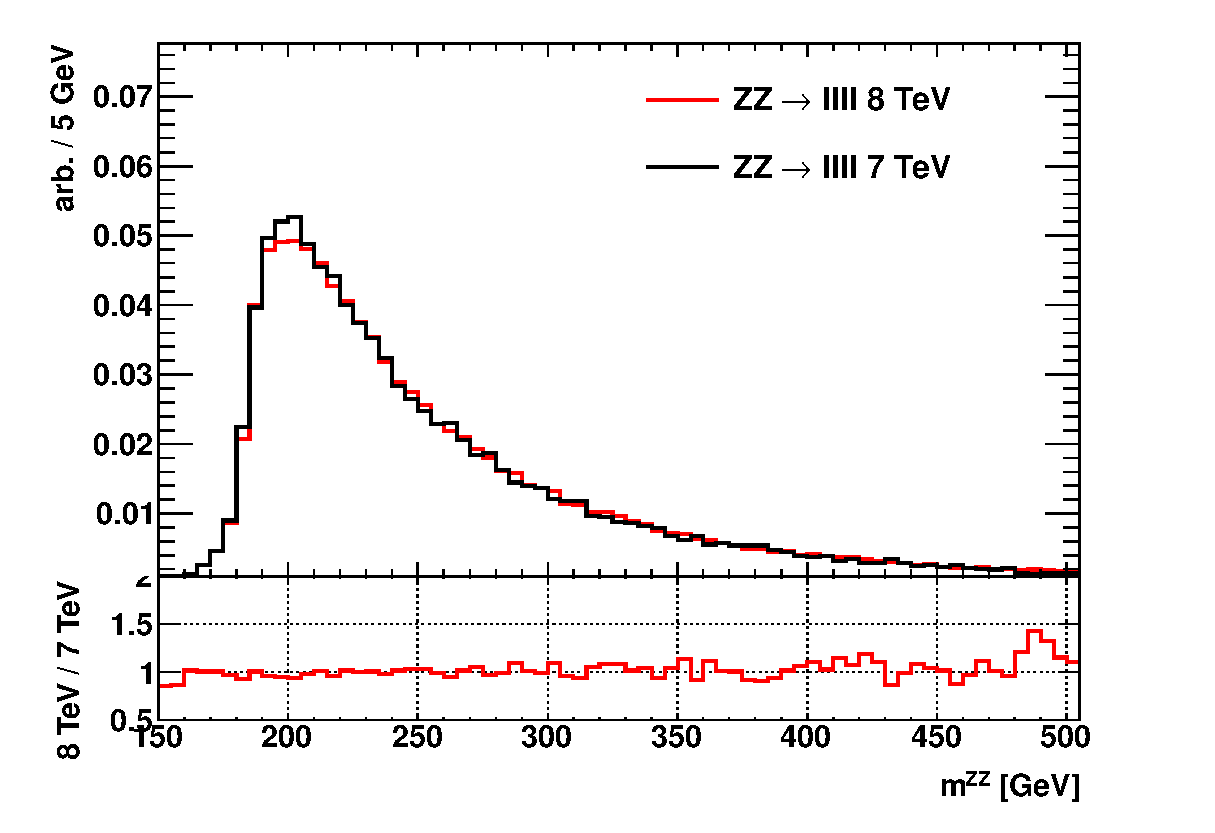
\includegraphics[width=0.32\textwidth]{truth_ZZ_ZZ_m_lin.eps}
    }
    \subfigure{
        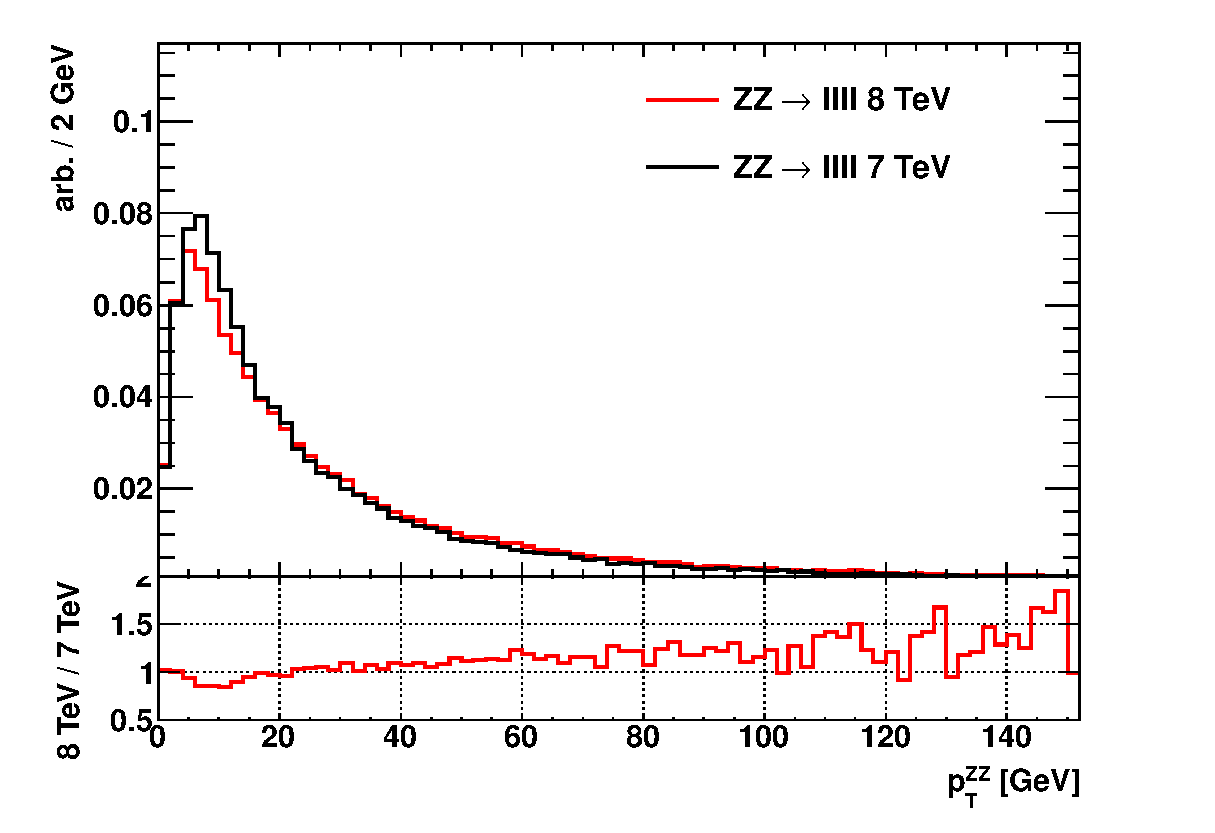
\includegraphics[width=0.32\textwidth]{truth_ZZ_ZZ_pt_lin.eps}
    }
    \subfigure{
        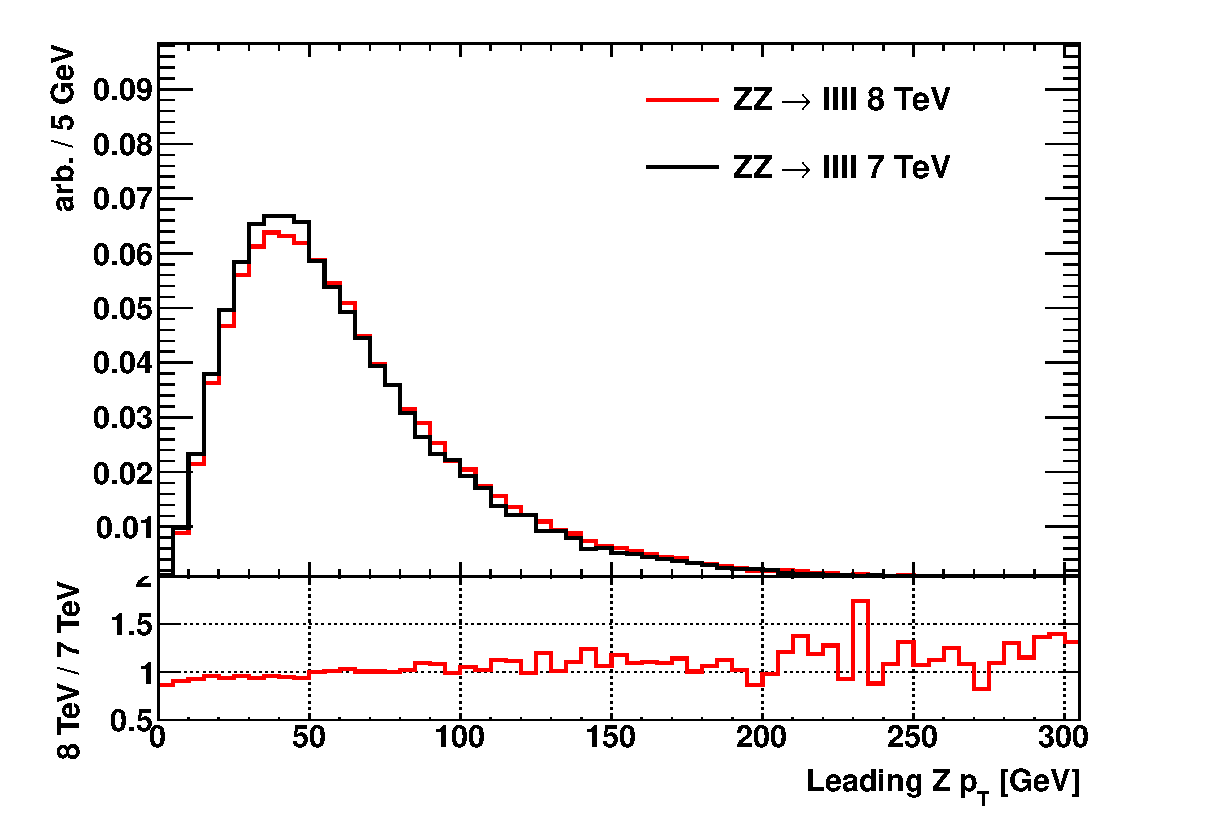
\includegraphics[width=0.32\textwidth]{truth_ZZ_Z1_pt_lin.eps}
    }
    \subfigure{
        \includegraphics[width=0.32\textwidth]{truth_ZZ_lep_1_pt}
    }
    \subfigure{
        \includegraphics[width=0.32\textwidth]{truth_ZZ_lep_1_eta}
    }
    \subfigure{
        \includegraphics[width=0.32\textwidth]{truth_ZZ_lep_4_pt}
    }
\end{figure}


%% TGC diagram
%\begin{figure}
%\centering
%        \vspace{10mm}
%    \mbox{
%    \subfigure{
%        \begin{fmffile}{schan}
%        \begin{fmfgraph*}(36,20)
%            \fmfleft{i1,i2}
%        \fmfright{o1,o2}
%        \fmflabel{$u,d$}{i2}
%        \fmflabel{$\bar{u},\bar{d}$}{i1}
%        \fmfright{o1,o2}
%        \fmflabel{$Z/\gamma^{*}$}{o1}
%        \fmflabel{$Z/\gamma^{*}$}{o2}
%        \fmf{fermion}{i2,v1,i1}
%        %\fmf{fermion}{v2,i2}
%        %\fmf{fermion}{v1,i1}
%        \fmf{photon,label=$Z/\gamma^{*}$}{v1,v2}
%        \fmf{photon}{v2,o1}
%        \fmf{photon}{v2,o2}
%        % uncommment this line if you want dots at the vertices
%            %\fmfdotn{v}{4}
%        \end{fmfgraph*}
%        \end{fmffile}
%    }
%    }
%        \vspace{5mm}
%    \caption{A diagram!}
%\end{figure}

%
\section{Previous experimental results}

Diboson ZZ production was first observed in $e^+e^-$ collisions at LEP in 1997.
The L3 experiment published the first observation and \cx\ measurement
of on-shell \ZZ\ production~\cite{Acciarri1999281}. They analysed 55.3 \ipb\
of data collected at an average centre-of-mass energy of 182.7 GeV. Separate
selections were applied in the various decay channels. Whilst no events were
observed in the $\ell\ell\ell\ell$ final states, a total of 63 were observed in
the other visible final states. The majority (47) of these were in the
all-hadronic channel, which suffered from high backgrounds from $e^+e-
\rightarrow qq \gamma$ and $e^+e- \rightarrow WW$. In this channel a neural
network method was used to distinguish the signal events from the background. A
log-likelihood fit of the neural network output and the observed mass spectra in
the other channels was used to combine the channels, and gave a \cx\ of
$\sigma_{ZZ} = 0.30^{+0.22 +0.07}_{-0.16 -0.03}$, in very good agreement with
the standard model prediction. The data were fitted to determine the magnitude
of the anomalous triple gauge couplings. These were found to be consistent with
the SM predictions of 0 to 95\% confidence level. Updated \cx\
measurements have since been published by L3 and the other 3 LEP experiments, in
all cases measuring \cx s for \ZZ\ production consistent with the
standard model, and finding no evidence for anomalous couplings.

Measurements of the \ZZ\ \cx\ have also been made in $p \bar{p}$
collisions at a centre of mass energy of $\sqrt{s} = 1.96$ \tev\ at the Tevatron, at
both the D0 and the CDF experiments. The most recent D0 publication reports the
observation of 10 candidate \ZZ\ events with an expected background of $0.37
\pm 0.13$. The measured \cx\ was $1.33^{+0.5}_{-0.4}$ (stat) $\pm$ 0.12
(syst) $\pm$ 0.09 (lumi) pb, with a signal significance of greater than
$6\sigma$. The result is consistent with the standard model prediction of 1.4
$\pm$ 0.1 pb. 

%The \cx\ at the LHC for a centre-of-mass energy of 7 \TeV\ is predicted to be $\sim$5 times larger 
%than at the Tevatron. 
Recently the CMS experiment have measured the \ZZ\ production cross
section~\cite{CMS-PAS-EWK-11-010} and found it consistent with the Standard Model prediction.


\section{Anomolous Triple Gauge Couplings}
Non-zero nTGCs would manifest as an increased \ZZ\
production \cx, especially at high \ZZ\ invarient mass and transverse
momentum~\cite{Baur:2000ae}.

\section{ZZ Resonances}
